\section*{Fragen aus der Vorbereitung}
\subsection*{a)}
	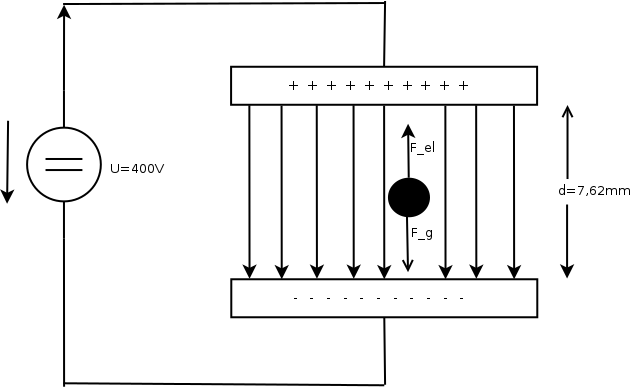
\includegraphics[scale=0.4]{Versuchsaufbau.png}
\subsection*{b)}
Für den Schwebefall müssen die Kraft der Gravitation und die Kraft des elektrischen Feldes gleich groß, mit gegenläufiger Wirkrichtung sein.
\[F_g = F_{el}\]
Die Erdanziehungskraft ist definiert als $F_g = m \cdot g$. Die Kraft mit der der Tropfen in Schwebe gehalten wird ist gegeben durch $F_{el} = \frac{U\cdot n \cdot q}{d} $. Da diese Betragsmäßig gleich sein müssen gilt:
\[m \cdot g  = \frac{U\cdot n \cdot q}{d}\]
Damit folgt für die Masse: $m = \frac{U\cdot n \cdot q}{d \cdot g}$.
\[m_{oel} = \frac{400V \cdot 2 \cdot 1,6 \cdot 10^{-19}C}{9,81\frac{m}{s^2} \cdot 7,62 \cdot 10^{-3}m} = 1,7123\cdot10^{-15}kg\]
\subsection*{c)}
Bei Verlust eines Elektrons wirkt nun nur noch die halbe elektrische Kraft auf den Öltropfen. Die Anziehungskraft der Erde ändert sich allerdings nicht. Damit ist die Erdanziehungskraft, die auf den Tropfen wirkt größer, als die ihr entgegen wirkende Kraft durch das elektrische Feld. Daraus folgt nun, dass der Tropfen zu Boden sinkt.
\subsection*{d)}
Ein Magnetfeld wirkt nur dann eine Kraft auf eine elektrische Ladung, wenn die Ladung sich bewegt, oder das Magnetfeld sich ändert. Der Fall könnte somit nicht aufgehalten werden. Da das Magnetfeld in die gleiche oder entgegengesetzte Richtung der Gravitationskraft wirk (beim Fall des Tropfens), wird der Tropfen weder verlangsamt, noch beschleunigt. Das Magnetfeld müsste senkrecht zur bewegten Ladung stehen, um eine Wirkung ausüben zu können.